% !TeX root = main.tex
\lecture{14}{Thu 05 Mar 2026 13:00}{Intro to Statistical Physics}

\section{Stefan-Boltzmann Law}
We can integrate across the whole spectrum to work out total energy emitted per unit time:
\[
    \dot{Q} = \epsilon \sigma A T^4
\]

Where $\sigma = 5.67 \times 10^{-8} \si{W m^{-2} K^{-1}}$ is the Stefan-Boltzmann constant, $\epsilon$ is the emissivity, $A$ is the surface area of the radiating body and $T$ is the temperature.


\section{Kinetic Theory of Gases}
We've now finished the module on temperature and move into statistical physics. We start wth a kinetic theory of the motion of gas molecules. Gas molecules move ``randomly'' (effectively, it's not computationally viable to determine what's actually going on), with vastly different velocities and positions.

We would love to describe a gas using the individual molecules that make it up, but that's really difficult to do for $\sim 10^{23}$ molecules so it's not viable and we have to use statistical physics to describe it.

We've previously touched upon the Maxwell-Boltzmann distribution to describe the velocities of particles as a statistical distribution wrt temperature:
\begin{figure}[H]
    \centering
    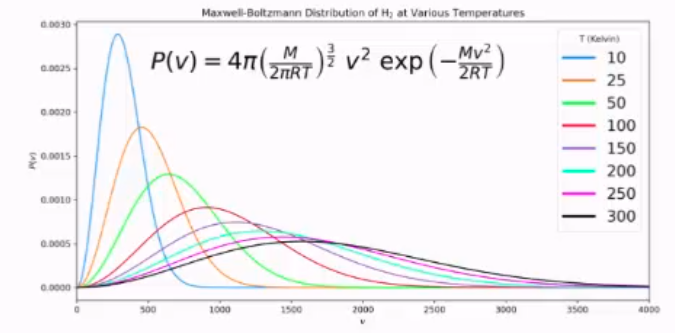
\includegraphics[width=\textwidth]{figures/lec07-1.png}
     \caption{}
\end{figure}

These statistical approximations improve as we increase the number of particles, and for very large numbers they become good approximations. We can in statistical physics have a probability $>1$. This seems mathematically strange, but we interpret it to mean that (if the probability represents the probability of an event occurring in a measurement), the event will take place multiple times. We still cannot have any probabilities $<0 $.

The rest of the lecture then turned into a fun tangent on statistics which isn't examinable and needs no notes.